\documentclass{scrartcl}
\usepackage{hyperref,listings}
\usepackage{tikz}
\usetikzlibrary{trees}

\lstset{ %
language=Matlab,                % the language of the code
basicstyle=\tt\small,       % the size of the fonts that are used for the code
%numbers=left,                   % where to put the line-numbers
%numberstyle=\footnotesize,      % the size of the fonts that are used for the line-numbers
%stepnumber=2,                   % the step between two line-numbers. If it's 1, each line 
                                % will be numbered
%numbersep=5pt,                  % how far the line-numbers are from the code
backgroundcolor=\color{white},  % choose the background color. You must add \usepackage{color}
showspaces=false,               % show spaces adding particular underscores
showstringspaces=false,         % underline spaces within strings
showtabs=false,                 % show tabs within strings adding particular underscores
%frame=single,                   % adds a frame around the code
tabsize=2,                      % sets default tabsize to 2 spaces
captionpos=b,                   % sets the caption-position to bottom
breaklines=true,                % sets automatic line breaking
breakatwhitespace=false,        % sets if automatic breaks should only happen at whitespace
title=\lstname,                 % show the filename of files included with \lstinputlisting;
                                % also try caption instead of title
escapeinside={\%*}{*)},         % if you want to add a comment within your code
morekeywords={*,...},           % if you want to add more keywords to the set
commentstyle=\color{green!50!black},
stringstyle=\color{red!50!blue}
}

\title{bcall-68}
\author{J\'er\^ome Boulanger}
\def\bs{\texttt{\backslash}}
\parindent=0pt
\begin{document}
\sf
\maketitle
\section{The big picture}
Bcall tries to perform a base calling by estimating the parameters of
a mixture of Gaussian. The element of the mixture are related to the
classes 00,01,10 and 11. The mixture parameters are estimated using
some additional constraints. The maximum a posteriori is found using
the well-know Expectation-Maximisation
algorithm\cite{em,em2}. Beforehand, a normalization of the data is
performed. The normalization can be done image-wise or/and
globally. Moreover, several normalization techniques can be
used. These one corresponds mainly to several methods for the
estimation of the center and the covariance of the data. The package
includes 3 different program with one having a graphical user
interface. 

\section{Using the 3 programs}

\subsection{bcall}

\texttt{bcall} performs the analysis of several datasets organized in
subfolders. For each dataset a 2 by 2 analysis is done and then a
global merge of the result is obtainted providing the final
results. Each subfolder should have a pair of log file with a
consistent number of objects and images.

In the command line window type (matlab or octave):

\texttt{>> [experiment, options]=bcall('Directory',options)}

\texttt{bcall} is a command line function for matlab that take two
parameters. The first one is the path to the \texttt{'Directory'}
containing SNP or CG sub-folders. The second one is an \texttt{options}
structure. Type \texttt{help bcall} in the commande window to get more
help. The function returns the experiment data and the options used.

\begin{table}
\label{tab:1}
\caption{Fields of the options structure for \texttt{bcall}. A boolean is true/false or 1/0}
\begin{center}
\begin{tabular}{llp{6cm}}
  name & values & description \\
  \hline
  \texttt{options.debug} & boolean & enable debug \\
  \texttt{options.cg} & string & pattern to match subdir names \\
  \texttt{options.normalization\_type} & $1,2,3,4$ & type of normalization. 1:none, 2:std, 3:robust std+median, 4:robust covariance+mean shift\\
  \texttt{options.beta} & float [0,1] & strenght of the constraints (the lower the stronger) \\
  \texttt{options.max\_cluster\_size}&float& target size for the clusters \\
  \texttt{options.imagewise\_normalization}&boolean& if \texttt{true} the normalization include a normalization image by image. This options is incompatible with pretrain\_bcall and  dysswitch\_bcall \\
  \texttt{options.remove\_bad\_image}&boolean& if \texttt{true} remove images which have too different nomalization parameters than the others \\
  \texttt{options.satellites} & boolean & tell if  \texttt{true} : use additionnal clusters \\
  \texttt{options.image}& list of integer & keep the specified images in the list. if equal -1 then all images are used.\\
  \texttt{options.pfiltercat}&float& minimal percentage of data dumped (not working for dyeswitch/pretrain\_bcall). \\
 \texttt{options.iterations}& integer & number of iterations. \\
\end{tabular}
\end{center}
\end{table}

\subsection{gbcall}

This is the graphical interface of \texttt{bcall}.

In the command line window type (matlab only):

\texttt{>> gbcall}

gbcall allows to graphically set the options of bcall and then call
bcall.
\begin{itemize}
\item \textbf{Data path:} Is used to locate the root of the folder
  where the data are stored (eg: Z:analysis).
\item \textbf{Directory:} Indicate the folder containing the
  subfolders (SNPs or CGs).
\item \textbf{Pattern:} The pattern allow to select the sub-folders in
  the folder ``directory''. A star means ``anything''. 
\item \textbf{Nucleotid:} Give a sequence of letter to indicate the
  nucleotids corresponding to the data. The sub-folder order is given
  by the operating system and the order of letters should correspond
  this order. For each sub-folder corresponds two nucleotids since
  each sub-folder contains two channels.
\item \textbf{Probability:} Set a threshod on the probability to
  belong to a class. 
\item \textbf{Iterations:} The EM algoritm is iterative. This set the
  number of iteration.
\item \textbf{Size cluster:} Is a constraint on the size of the
  clusters, when set to 0, no constraint is applied. The effect of
  this parameter has been changed a lot since the previous
  version. Default value is now 0 (no constraints).
\item \textbf{Filter output:} Threshold to remove classes with less
  points than a certain percent of the all data set.
\item \textbf{Image:} Select a specific image to perform the analysis.
\item \textbf{Satellites:} Enable the use of additional cluster to
  represent the 00 class.
\item \textbf{Debug:} Enable the debug mode.
\item \textbf{Final plotting:} Enable the plotting of the global graph
  (time consumming).
\item \textbf{Close figures:} Close figure before starting the
  analysis.
\item \textbf{Imagewise normalization:} Normalize each image using a
  robust variance (MAD) estimation and the median. This is dangerous
  when data have less than 50\% of points in class 00.
\item \textbf{Remove bad images:} Remove image whose points are
  statistically different from the average (based on mean and
  variance).
\item \textbf{Normalization:} Select a normalization
  (options.normalization\_type):
\begin{enumerate}
\item none: no normalisation.
\item standard : use the mean and standard deviation given by
  \texttt{mean} and \texttt{std} from matlab. Usually performs poorly
  due to the outliers (\cite{outliers}) corresponding to the class 10,01,11.
\item MAD/Med : use the median absolute deviation \cite{mad} and the median
  (robust up to 50\% of outliers) 
\item MDL/MS : use MDL criterion to estimate the covariance matrix and
  a mean shift to locate the lower left mode. This approach is more
  robust and can be used in cases where the 00 cluster is less than
  50\%.
\item same as previous but use the covariance matrix to whiten the data.
\end{enumerate}
\item \textbf{Save:} Save parameters
\item \textbf{Reset:} Reset to default (saved) parameters.
\item \textbf{Ok:} Launch the base calling.
\end{itemize}

\subsection{pretrain\_bcall}
It is a \emph{command line program} (there is no graphical user
interface for this program) which perform the analysis of several
files in distinct directories which are name following the pattern
\texttt{options.cg} using the \emph{same} parameters estimated globally or on
the first dataset. This program allow to analyse a set of several
folders containing each a pair of file w2/w3 (or w4/w5
etc\dots). Accordingly, the files should be organized as in
Figure~\ref{fig:1}. The experiments do not necesseraly have the same
number of beads/objects/images.

\begin{figure}
\begin{center}
\begin{tikzpicture}[every node/.style={draw=black,fill=yellow!25},level distance=.75cm,level 1/.style={sibling distance=2cm},level 2/.style={sibling distance=1cm},font=\footnotesize]
\node at (-4,1) {MyFolder}
child {node {SubFolder1} child {node {w2}} child {node {w3}}}
child {node {SubFolder2} child {node {w2}} child {node {w3}}}
child {node {SubFolder3} child {node {w2}} child {node {w3}}};
% \end{tikzpicture}
% 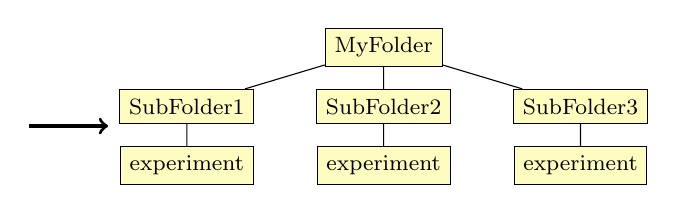
\begin{tikzpicture}[every node/.style={draw=black,fill=yellow!25},level distance=.75cm,level 1/.style={sibling distance=2.5cm},level 2/.style={sibling distance=1cm},font=\footnotesize]
\draw[->,very thick] (-.5,0)--(.5,0);
\node at (4,1) {MyFolder}
child {node {SubFolder1} child {node {experiment}} }
child {node {SubFolder2} child {node {experiment}} }
child {node {SubFolder3} child {node {experiment}} };
\end{tikzpicture}
\end{center}
\caption{Two possible organizations of files in \texttt{bcall} and
  \texttt{pretrain\_bcall}. The folders can contains other
  files. The first case is before any processing, while the second
  correspond to the state of the folder after it has been loaded once.}
\label{fig:1}
\end{figure}

The command line window type (matlab or octave) usage is:

\texttt{>> [experiment,options]=pretrain\_bcall('Directory',options)}

You can also use it as :

\texttt{>> pretrain\_bcall('Directory',options)}


The arguments of the program are 
\begin{itemize}
\item \textbf{'Directory'} is a string indicating the path to the folder
  where are the data, please do not forget that a string is
  constructed using quotes, eg
  \texttt{'Z:{\textbackslash}Analysis{\textbackslash}...'}.
\item \textbf{options} is a structure containing options (see
  Table~\ref{tab:1}). In addition, set \texttt{options.global=true} to
  enable the analysis of the datasets globally (merging all the data,
  normalizing and estimating the parameters of the mixture) or using
  only the data set from the 1st file. By default
  \texttt{options.global=false}.
\end{itemize}

For example, in the console window:
\begin{lstlisting}
directory='Z:\Analysis\MyFolder\'; % containing SubFolder1 SubFolder2 SubFolder3
options.cg='/SubFolder*'; % this is compulsory unless it is  'SNP*'
options.max_cluster_size=1.5; % Define the cluster size
options.beta=0.1; % set the strengh of the constraint (small is strong)
options.satellites=true; % will use satellites
options.remove_bad_images=true; % will remove bad images
options.global=false; % will use only the 1st image to calibrate the analysis
pretrain_bcall(directory,options); % finally lauch the analysis
\end{lstlisting}


\subsection{dyeswitch\_bcall}
Command line which performs the analysis of a dye switch
experiment. The set of experiments share the same number of
images/objects. The calibration is learned by default on the merged
datas (globally : \texttt{options.global=true}).

The command line window type (matlab or octave) usage is:

\texttt{>> [experiment,options]=dyeswitch\_bcall('Directory',options);}

You can also use it as :

\texttt{>> dyeswitch\_bcall('Directory',options);}
The arguments of the program are 
\begin{itemize}
\item \textbf{'Directory'} is a string indicating the path to the folder
  where are the data, please do not forget that a string is
  constructed using quotes, eg
  \texttt{'Z:{\textbackslash}Analysis{\textbackslash}...'}.
\item \textbf{options} is a structure containing options (see
  Table~\ref{tab:1}).
\end{itemize}

For example, in the console window:
\begin{lstlisting}
directory='Z:\Analysis\MyFolder\'; % containing SubFolder1 SubFolder2 SubFolder3
options.cg='/SubFolder*'; % this is compulsory unless it is  'SNP*'
options.max_cluster_size=1.5; % Define the cluster size
options.beta=0.1; % set the strengh of the constraint (small is strong)
options.satellites=true; % will use satellites
options.remove_bad_images=true; % will remove bad images
options.global=false; % will use only the 1st image to calibrate the analysis
dyeswitch_bcall(directory,options); % finally lauch the analysis
\end{lstlisting}

\section{Two steps analysis}
The two functions \texttt{calibration} and \texttt{apply} allows to
perform the analysis in two steps. First estimating the parameters and
then applying the classification.
\begin{lstlisting}
% Step 1
directory1='Z:\Analysis\MyFolder1\'; % containing the calibration datasets
options.cg='/SubFolder*'; % this is compulsory unless it is  'SNP*'
options.max_cluster_size=1.5; % Define the cluster size
options.beta=0.1; % set the strengh of the constraint (small is strong)
options.satellites=true; % will use satellites
options.remove_bad_images=true; % will remove bad images
options.global=true; % will use only the 1st image to calibrate the analysis
options=calibration(directory1,options);
save('mycalibration.mat','options'); % eventually save the calibation

% Step 2
options = load('mycalibration.mat'); % and restore it later
directory1='Z:\Analysis\MyFolder2\'; % containing the folders to analyze
apply(directory1,options); % apply the calissifiaction and save the results
\end{lstlisting}

\bibliographystyle{plain}
\begin{thebibliography}{2}

\bibitem[1]{em} Dempster, A.P.; Laird, N.M.; Rubin,
  D.B. (1977). "Maximum Likelihood from Incomplete Data via the EM
  Algorithm". Journal of the Royal Statistical Society. Series B
  (Methodological) 39 (1): 1–38.

\bibitem[2]{em2} \url{http://en.wikipedia.org/wiki/Expectation-maximization\_algorithm}

\bibitem[3]{outliers} \url{http://en.wikipedia.org/wiki/Outlier}
   
\bibitem[4]{mad} \url{http://en.wikipedia.org/wiki/Median\_absolute\_deviation}

\end{thebibliography}

\end{document}

%%% Local Variables:  
%%% mode: tex-pdf
%%% End:
